\documentclass[norsk,a4paper,12pt]{article}
\usepackage[utf8]{inputenc}
\usepackage{graphicx} %for å inkludere grafikk
\usepackage{verbatim} %for å inkludere filer med tegn LaTeX ikke liker
\usepackage{tabularx}
\usepackage{booktabs}
\usepackage{amsmath}
\usepackage{float}
\usepackage{color}
\usepackage{listings}
\usepackage{physics}
\usepackage{hyperref}
\lstset{language=c++}
\lstset{basicstyle=\small}
\lstset{backgroundcolor=\color{white}}
\lstset{frame=single}
\lstset{stringstyle=\ttfamily}
\lstset{keywordstyle=\color{red}\bfseries}
\lstset{commentstyle=\itshape\color{blue}}
\lstset{showspaces=false}
\lstset{showstringspaces=false}
\lstset{showtabs=false}
\lstset{breaklines}
\lstset{postbreak=\raisebox{0ex}[0ex][0ex]{\ensuremath{\color{red}\hookrightarrow\space}}}
\usepackage{titlesec}

\setcounter{secnumdepth}{4}

\titleformat{\paragraph}
{\normalfont\normalsize\bfseries}{\theparagraph}{1em}{}
\titlespacing*{\paragraph}
{0pt}{3.25ex plus 1ex minus .2ex}{1.5ex plus .2ex}


\title{FYS3150 - Computational Physics\\\vspace{2mm} \Large{Project 5}}
\author{\large Richard Andr\'e Fauli\\ Dorthea Gjestvang\\ Even Marius Nordhagen}
\date{December 24, 2016}
\begin{document}

\maketitle
\begin{abstract}
This project aims to simulate so-called quantum dots, electrons trapped in harmonic oscillator potentials, by
\end{abstract}


\begin{itemize}
\item Github repository containing programs and results are in: \url{https://github.com/richaraf/Comphys_projects/tree/master/Project_5}
\end{itemize}


\section{Introduction}
In this project, we study the theory behind quantum dots, a highly relevant subject in modern physics. A quantum dot is one or two electrons trapped in an quantum well. These are often referred to as arificial atoms, as they, like natural atoms, have discrete energy levels \cite{Nature}.

Our goal in this project is to simulate a quantum dot, modelled as one or two electrons bound in a three-dimensional harmonic oscillator well, both with and without Coulomb interaction.


\section{Theory}

\subsection{Variational Method} \label{VariationalMethod}
The variational method is a method in quantum mechanics for estimating an upper limit on the lowest energy state level for a given Hamiltonian \cite{Griffiths}. For any choice of wave function $\Psi$, the following expression holds:

\begin{equation}
    E_0 \leq \frac{\bra{\Psi} H \ket{\Psi}}{\bra{\Psi}\ket{\Psi}} = E_T
    \label{eq:VariationalMethod}
\end{equation}

where $E_T$ is the trial energy. 
Equation \ref{eq:VariationalMethod} states that given a wave function $\Psi$, the calculated expectation value for the energy $E_T$ will always be greater than or equal to the lowest energy, $E_0$. This is trivial to understand: if the chosen $\Psi$ indeed is the ground state $\Psi_0$, then the trial energy is $E_0$. For any other choice of $\psi$, the trial  energy must be higher than the energy of the ground state. \par 
The variational method is particularly useful when the Hamiltonian has complicated eigenfunctions, or no analytical solution at all. A smart choice of a trial wave function $\Psi_T(\alpha)$ where $\alpha$ is the variational parameter, gives the trial energy $E_T(\alpha)$, which is an upper limit on the ground state energy as a function of $\alpha$. The trial energy can thereafter be minimized with respect til $\alpha$, giving an upper limit to $E_0$ that is as low as possible.

\subsection{Quantum Dot Model}
As stated in the introduction, we simulate a quantum dot as two electrons in a three dimensional harmonic oscillator well. We will both simulate the electrons when neglecting Coulomb interaction between the two electrons, and when including this repulsion. For the non-interacting case, the Hamiltonian $\hat{H}$ is:

\begin{equation}
    \hat{H} = \sum_{i=1}^{2} (-\frac{\hbar^2}{2 m_e}\nabla_i^2 + \frac{1}{2}\hbar \omega^2r_i^2) 
    \label{eq:H_non_interaction_unit}
\end{equation}

where the sum goes over all particles $i$, $\nabla_i^2$ is the Laplace operator for particle $i$, $\omega$ is the harmonic well frequency and $r_i$ is the position vector of particle $i$. 

For the interacting case, the electrons notices a repulsion from the Coulomb interaction, and we have to include an additional term in the Hamiltonian:

\begin{equation}
    \hat{H_{rep}} = \sum_{i<j} \frac{e^2}{4\pi \epsilon_0 r_{ij}}
    \label{eq:H_interaction_unit}
\end{equation}

where $r_{ij}$ is the distance between electron $i$ and $j$, $e$ is the elementary charge, $\epsilon_ 0$ is the permittivity of vacuum, and we sum over $i < j$ to avoid counting interactions twice, as the potential from electron $i$ acting on $j$ is the same as the potential from $j$ acting on $i$. Using natural units, that is scaling such that $\hbar = e = m_e = 1$ and $\epsilon_0 = \frac{1}{4\pi}$, we obtain the scaled Hamiltonians for the non-interacting and the interacting system presented in equation (\ref{eq:H_non_interaction}) and (\ref{eq:H_interaction}):

\begin{equation}
    \hat{H} = \sum_{i=1}^{2} (-\frac{1}{2}\nabla_i^2 + \frac{1}{2} \omega^2r_i^2) 
    \label{eq:H_non_interaction}
\end{equation}

\begin{equation}
    \hat{H_{rep}} = \sum_{i<j} \frac{1}{r_{ij}}
    \label{eq:H_interaction}
\end{equation}

We wish to find estimates for the ground state energy using the variational method, presented in subsection \ref{VariationalMethod}. For this, we will use the trial wave functions presented in equation (\ref{eq:PsiT1}) and (\ref{eq:PsiT2}):

\begin{equation}
    \Psi_{T1} (r_1, r_2) = Ce^{-\alpha \omega (\frac{r_1^2 + r_2^2}{2})}
    \label{eq:PsiT1}
\end{equation}

\begin{equation}
    \Psi_{T2}(r_1, r_2) = Ce^{-\alpha \omega (\frac{r_1^2 + r_2^2}{2})}e^{\frac{r_{12}}{2(1+\beta r_{12})}}
    \label{eq:PsiT2}
\end{equation}

where C is a normalization constant and $\beta$ is a variational parameter. We will use the variational method with $\Psi_{T1}$ on the non-interaction Hamiltonian in equation (\ref{eq:H_non_interaction}), and $\Psi_{T2}$ with the interaction Hamiltonian in equation (\ref{eq:H_non_interaction}) + (\ref{eq:H_interaction}).

\subsection{Energies} \label{Energies}
In order to find the local energy $E_L$ for a given trial function $\Psi_T$ we can use the following expression
\begin{equation}
E_L = \frac{1}{\Psi_T}\hat{H}\Psi_T,
\label{eq:localenergy}
\end{equation}

where $\hat{H}$ is the Hamiltonian. Using equation (\ref{eq:localenergy}) and the first trial wave function (\ref{eq:PsiT1}) we get the local energy to be

\begin{equation}
E_{L1} = \frac{1}{2}\omega^2 (r_1^2 + r_2^2)(1-\alpha^2) + 3\alpha \omega,
\label{eq:EL1}
\end{equation}

which contains both kinetic $T_1$ and potential $V_1$ energy

\begin{equation}
T_1 = 3\alpha \omega -\frac{1}{2}\omega^2\alpha^2\left(r_1^2 + r_2^2\right),
\label{eq:T_1}
\end{equation}

\begin{equation}
V_1 = \frac{1}{2}\omega^2(r_1^2 + r_2^2).
\end{equation}

\section{Method}

\subsection{Implementation}

When implementing the code, we made separate classes for $\Psi_{T1}$ and $\Psi_{T2}$, with their respective analytical energies as member functions. \par 
\vspace{2mm}

Our trial wave functions are functions of $\vec{r_1}$ and $\vec{r_2}$, and we give our system a random initial state. As both our trial wave functions are proportional to $e^{-\alpha \omega}$, a natural length scale for our system is $\frac{1}{\sqrt{\omega}}$, as the wave function dies out after $\pm \frac{1}{\sqrt{\omega}}$. We therefore choose a random initial position that is an random number $ random\_number \in [0,1]$, times the length scale for each of the three direction:

\begin{equation}
    position =  random\_number \cdot length\_scale
    \label{random_steps}
\end{equation}

Thereafter, we loop over a number of Monte Carlo Cycles, for each cycle suggesting a random movement for one of the electrons. This random movement follows the same pattern as the generation of the initial position, from equation (\ref{random_steps}). This move is accepted or rejected through the Metropolis algorithm with the probability distribution $|\Psi_T|^2$, presented in subsection \ref{MetropolisAlgorithm}. This way, we can use Monte Carlo Integration for calculating the energy for integration points drawn from our PDF and after $N$ Monte Carlo cycles, we can calculate the trial energy $E_T$.

\subsection{Monte Carlo Integration}
In our project, we will use Monte Carlo Integration. The brute-force way of doing Monte Carlo integration is approximating the integral as a sum, as presented in equation (\ref{eq:MC_int_bruteforce}):

\begin{equation}
    \int_0^1 f(x) dx \approx  \frac{1}{N}\sum_{i=0}^N f(x_i) \quad x \in [0,1]
    \label{eq:MC_int_bruteforce}
\end{equation}

where $f(x)$ is the function we want to integrate and N is the number of integration points. 

A smarter way of doing Monte Carlo integration, is writing the function $f(x)$ as a $g(x)\cdot PDF$ where $PDF$ is a probability distribution, and $g(x)$ is the remaining parts of $f(x)$. Instead of drawing the integration points $x_i$ entirely at random, we can draw them from the PDF, as presented in equation (\ref{MC_int_prob}):

\begin{equation}
    \frac{1}{N}\sum_{i=0}^N g(x_i) PDF \quad x_i \in [-\infty, \infty] \Rightarrow \frac{1}{N} \sum_{i=0}^N g(x_i) \quad x_i \sim PDF
    \label{MC_int_prob}
\end{equation}

This is a more efficient way of doing Monte Carlo integration, as the integration points $x_i$ are chosen from the interval where the function $g(x)$ is interesting.\par 

In our project, we wish to calculate the trial energy, given by equation (\ref{eq:VariationalMethod}). If we rewrite the energy as the local energy $E_L$ from equation (\ref{eq:localenergy}), we can rewrite the inner product as the local energy multiplied with $|\Psi_T|^2$:

\begin{equation}
    \int \Psi_T^* H \Psi_T dV = \int E_L |\Psi_T|^2 dV \Rightarrow \frac{1}{N} \sum_{i=0}^N E_L(x_i) \quad x_i \sim |\Psi_T|^2  
\end{equation}

From quantum mechanics, we know $|\Psi_T|^2$ is the probability density of finding a system in a given interval. 

The method of drawing random numbers from a probability distribution is the Metropolis Algorithm, presented in \ref{MetropolisAlgorithm}. 

The implementation is as follows:

\begin{lstlisting}
    E_tot = 0
    
    #N Monte Carlo Cycles
    for(n=0, n < N, n++):
        calculate E_L from function, choose integral points from PDF
        E_tot += E_L
        
    E = E_tot/N
        
    
\end{lstlisting}

\subsection{Metropolis Algorithm} \label{MetropolisAlgorithm}
We wish to draw random numbers from a PDF, and in our program this PDF is $|\Psi_T|^2$. For this, we use the Metropolis algorithm. We know that the electrons is more likely to be found at higher probability density values, i e larger values of $|\Psi_T|^2$. If the factor $|\Psi_T|^2$ increases when randomly changing one of the electron's position, the algorithm should automatically accept this move. The move should also be accepted if $|\Psi_T|^2$ remains constant.

\par 
\vspace{2mm}

If the probability density decreases, however, this should be allowed, but not probable. Our program calculates the factors $|\Psi_T_{old}|^2$ and $|\Psi_T_{new}|^2$ for the old and new positions respectively, and their ratio $ m = \frac{|\Psi_T_{new}|^2}{|\Psi_T_{old}|^2}$, which is less than $1$. Thereafter, the program draws a random number $p$ in the interval $\in [0, 1]$, and compares the ratio $m$ with the random number $k$. If $m \geq k$, the move is accepted. If the $m < k$ the move of the electron is rejected, and the system is reset to the old position. 

\par 
\vspace{3mm}

The implementation would look like the following:

\begin{lstlisting}
    
    Psi_T_old_squared #calculate from function
    
    r_new[i] = r_old[i] + length_scale*random_number
    
    Psi_T_new_squared #calculate from function
    
    if(Psi_T_new_squared > Psi_T_old_squared):
        accept
    
    else:
        m = Psi_T_new_squared/Psi_T_old_squared
        k = random number in [0,1]
        
        if(m >= k):
            accept
            
        else:
            deny, reset to old positions
    
    
    
    
\end{lstlisting}

\section{Results}
\subsection{$\Psi_{T1}$}

We used the trial wave function $\Psi_{T1}$, given by equation (\ref{eq:PsiT1}), and plotted the energies and the variance in energy as a function of $\alpha$ for different values of $\omega$. The results are shown in Figure \ref{fig:E_L1_file_omega=1_0} - \ref{fig:E_L1_file_omega=0_01}.

\begin{figure} [H]
    \centering
    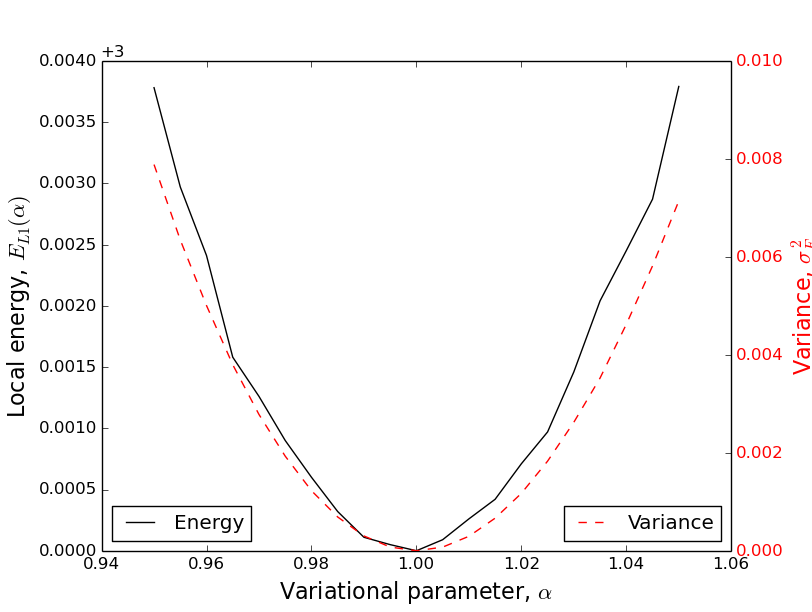
\includegraphics[scale=0.65]{E_L1_variance_omega=1_0}
    \caption{Local energy and variance plotted  for $\Psi_{T1}$ as a function of $\alpha$, for $\omega = 1.0$. We observe that $\alpha = 1.0$ gives the energy $E=3.0$ }
    \label{fig:E_L1_file_omega=1_0}
\end{figure}


\begin{figure} [H]
    \centering
    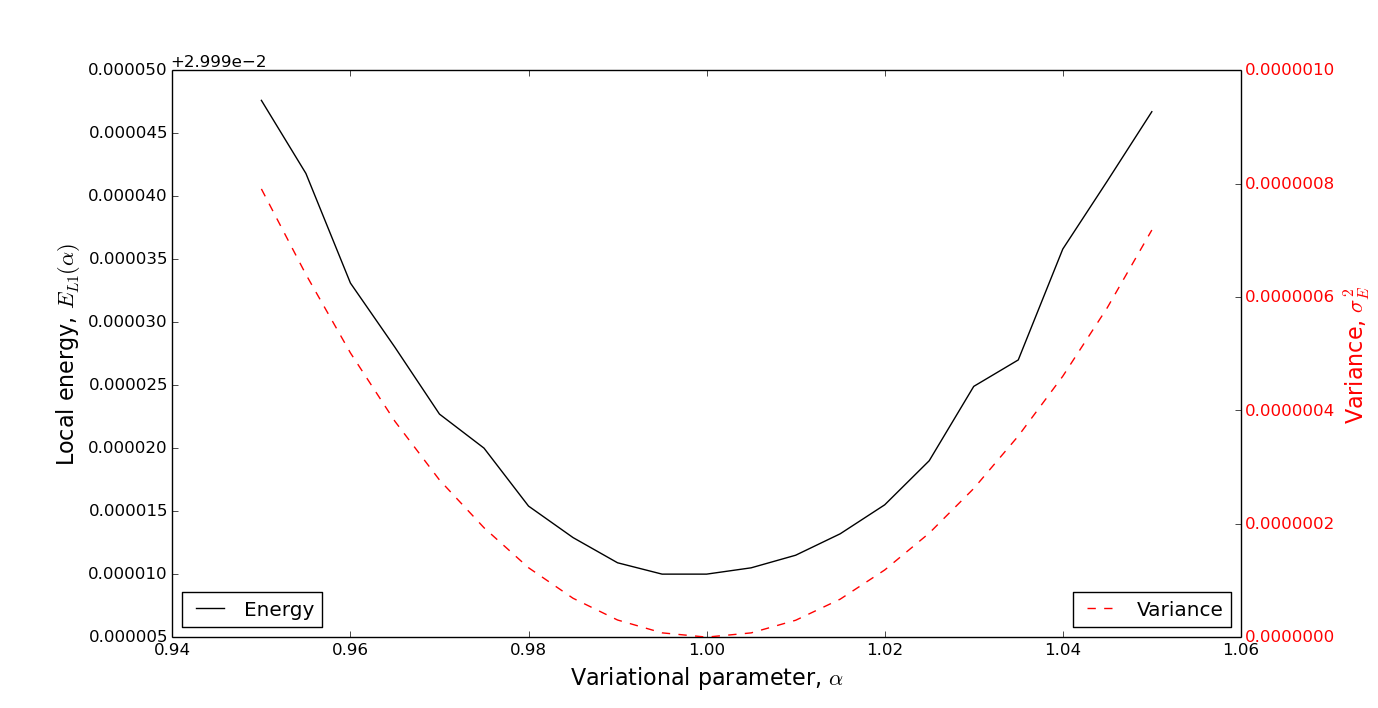
\includegraphics[scale=0.65]{E_L1_variance_omega=0_01}
    \caption{Local energy and variance plotted  for $\Psi_{T1}$ as a function of $\alpha$, for $\omega = 0.01$. We observe that $\alpha = 1.0$ gives the energy $E=3.0$, FEIL PLOTT, fiks på nytt }
    \label{fig:E_L1_file_omega=0_01}
\end{figure}

We also calculated the average distance between the two electrons for the optimal value of $\alpha$, for different values of $\omega$. The results are presented in Table 

\begin{table} [H]
\centering
\caption{The average distance between the two electrons for $\Psi_{T1}$, for different values og $\omega$.}

\begin{tabularx}{\textwidth}{XXXX} \hline
\label{2x2Lattice_Microstates}
{\bf } & {\bf $\omega = 1.0$ } & {\bf $ \omega = 0.5 $ } & {\bf $\omega = 0.01$} \\ \hline
{$r_{12}$} & & & &\\ \hline 
\end{tabularx}
\end{table}


\section{Discussion}
\section{Conclusion}

\newpage
\section{References}
\begingroup
\renewcommand{\section}[2]{}
\begin{thebibliography}{}
\bibitem{Nature}
  R C Asgoori. 
  Electrons in artificial atoms
  Nature Vol 379 1.February 1996
  \url{http://www.nature.com/nature/journal/v379/n6564/pdf/379413a0.pdf}
\bibitem{Griffiths}
  D J Griffiths (2014)
  Introdction to Quantum Mechanics, Second Edition
  
  

\end{thebibliography}

\end{document}
